%%
%% This is file `sample-sigchi-a.tex',
%% generated with the docstrip utility.
%%
%% The original source files were:
%%
%% samples.dtx  (with options: `sigchi-a')
%%
%% IMPORTANT NOTICE:
%%
%% For the copyright see the source file.
%%
%% Any modified versions of this file must be renamed
%% with new filenames distinct from sample-sigchi-a.tex.
%%
%% For distribution of the original source see the terms
%% for copying and modification in the file samples.dtx.
%%
%% This generated file may be distributed as long as the
%% original source files, as listed above, are part of the
%% same distribution. (The sources need not necessarily be
%% in the same archive or directory.)
%%
%% The first command in your LaTeX source must be the \documentclass command.

%% Starting in 2020, ACM retired formats sigchi and
%% sigchi-a. SIGCHI conferences now use sigconf format for
%% their publications. If a file uses sigchi format, a
%% warning is issued, and the format is automatically
%% switched to sigconf. Format sigchi-a can be used for
%% non-ACM documents only.
\documentclass[sigchi-a,nonacm]{acmart}

%Custom packages
\usepackage{microtype}

%% Anonymous
% \documentclass[sigchi-a,nonacm,anonymous=true]{acmart}
%%
%% \BibTeX command to typeset BibTeX logo in the docs
\AtBeginDocument{%
  \providecommand\BibTeX{{%
    \normalfont B\kern-0.5em{\scshape i\kern-0.25em b}\kern-0.8em\TeX}}}
    

%% Rights management information.  This information is sent to you
%% when you complete the rights form.  These commands have SAMPLE
%% values in them; it is your responsibility as an author to replace
%% the commands and values with those provided to you when you
%% complete the rights form.
\setcopyright{acmcopyright}
\copyrightyear{2021}
\acmYear{2021}
\acmDOI{unknown}

%% These commands are for a PROCEEDINGS abstract or paper.
\acmConference[CIU@IUI 2021]{Woodstock '18: ACM Symposium on Neural
  Gaze Detection}{June 03--05, 2011}{Woodstock, NY}
\acmBooktitle{Woodstock '18: ACM Symposium on Neural Gaze Detection,
  June 03--05, 2018, Woodstock, NY}
\acmPrice{15.00}
\acmISBN{978-1-4503-XXXX-X/18/06}


%%
%% Submission ID.
%% Use this when submitting an article to a sponsored event. You'll
%% receive a unique submission ID from the organizers
%% of the event, and this ID should be used as the parameter to this command.
%%\acmSubmissionID{123-A56-BU3}

%%
%% The majority of ACM publications use numbered citations and
%% references.  The command \citestyle{authoryear} switches to the
%% "author year" style.
%%
%% If you are preparing content for an event
%% sponsored by ACM SIGGRAPH, you must use the "author year" style of
%% citations and references.
%% Uncommenting
%% the next command will enable that style.
%%\citestyle{acmauthoryear}

%%
%% end of the preamble, start of the body of the document source.
\begin{document}

%%
%% The "title" command has an optional parameter,
%% allowing the author to define a "short title" to be used in page headers.
\title{Take Back Control: User Privacy and Transparency Concerns in Personalized Conversational Agents}

%%
%% The "author" command and its associated commands are used to define
%% the authors and their affiliations.
%% Of note is the shared affiliation of the first two authors, and the
%% "authornote" and "authornotemark" commands
%% used to denote shared contribution to the research.
% \author{anon}
% \authornote{}
% \email{ana}
% \orcid{}
% \author{}
% \authornotemark[1]
% \email{}
% \affiliation{%
%   \institution{Institute for Clarity in Documentation}
%   \streetaddress{P.O. Box 1212}
%   \city{Dublin}
%   \state{Ohio}
%   \postcode{43017-6221}
% }
\author{Iris Hendrickx}
% \authornotemark[1]
\affiliation{%
  \institution{Centre for Language Studies, Centre for Language and Speech Technology, Radboud University}
  \streetaddress{Erasmusplein 1}
  \city{Nijmegen}
  \postcode{6500 HD}
  \country{The Netherlands}}
\email{i.hendrickx@let.ru.nl}

\author{Jelte van Waterschoot}
% \authornote{Both authors contributed equally to this research.}
\affiliation{%
  \institution{Human Media Interaction, \\ University of Twente}
  \streetaddress{Drienerlolaan 5}
  \city{Enschede}
  \country{The Netherlands}
  \postcode{7522 NB}}
\email{j.b.vanwaterschoot@utwente.nl}
  \orcid{0000-0002-3361-2105}

%\author{Helmer Strik}
%\affiliation{%
%  \institution{Centre for Language and Speech Technology, Radboud University}
 % \streetaddress{Erasmusplein 1}
 % \city{Nijmegen}
 % \postcode{6500 HD}
 % \country{The Netherlands}}
 % \email{w.strik@let.ru.nl}

\author{Arif Khan, Louis ten Bosch}
\affiliation{%
  \institution{Centre for Language Studie,Centre for Language and Speech Technology, Radboud University}
  \streetaddress{Erasmusplein 1}
  \city{Nijmegen}
  \postcode{6500 HD}
  \country{The Netherlands}}
\email{{a.khan;l.tenbosch}@let.ru.nl}

\author{Helmer Strik, Catia Cucchiarini}
\affiliation{%
  \institution{Centre for Language Studie, Centre for Language and Speech Technology, Radboud University}
  \streetaddress{Erasmusplein 1}
  \city{Nijmegen}
  \postcode{6500 HD}
  \country{The Netherlands}}
\email{{w.strik;c.cucchiarini}@let.ru.nl}

%%
%% By default, the full list of authors will be used in the page
%% headers. Often, this list is too long, and will overlap
%% other information printed in the page headers. This command allows
%% the author to define a more concise list
%% of authors' names for this purpose.
\renewcommand{\shortauthors}{Hendrickx et al.}

%%
%% The abstract is a short summary of the work to be presented in the
%% article.
\begin{abstract}
We reflect on user privacy concerns, transparency and informed consent for long-term interactions with personalized conversational agents.
We argue that the common practice of asking users to sign an informed consent form is insufficient to accommodate the privacy concerns of the user. We propose that long-term engaging personalized conversational agents must include an explicit mechanism in %their conversations to allow users to for control and transparency of stored personal information.
their conversations to allow users to have better control over their stored personal information and to have transparency about who is allowed to view the stored personal information.
\end{abstract}

%%
%% The code below is generated by the tool at http://dl.acm.org/ccs.cfm.
%% Please copy and paste the code instead of the example below.
%%
\begin{CCSXML}
<ccs2012>
   <concept>
       <concept_id>10002978.10003029.10003032</concept_id>
       <concept_desc>Security and privacy~Social aspects of security and privacy</concept_desc>
       <concept_significance>500</concept_significance>
    </concept>
    <concept>
        <concept_id>10003120.10003121.10003122.10003332</concept_id>
        <concept_desc>Human-centered computing~User models</concept_desc>
        <concept_significance>300</concept_significance>
    </concept>
    <concept>
       <concept_id>10003120.10003138.10003141.10010900</concept_id>
       <concept_desc>Human-centered computing~Personal digital assistants</concept_desc>
       <concept_significance>300</concept_significance>
   </concept>
</ccs2012>
\end{CCSXML}
\ccsdesc[500]{Security and privacy~Social aspects of security and privacy}
\ccsdesc[300]{Human-centered computing~User models}
\ccsdesc[300]{Human-centered computing~Personal digital assistants}


%% Keywords. The author(s) should pick words that accurately describe
%% the work being presented. Separate the keywords with commas.
\keywords{conversational agents, privacy concerns, user consent, personalization}


%%
%% This command processes the author and affiliation and title
%% information and builds the first part of the formatted document.
\maketitle

%%%%%%%%%%%%%%%%%%
% Introduction
%%%%%%%%%%%%%%%%%%
\section{Introduction} 
%Outline paper for Intelligent User Interface workshop: %http://speechinteraction.org/IUI2021/callforpapers.html
%Context of this paper: personal information, spoken interaction, conversational agents, transparancy, privacy

%The goal of our research project \emph{Behaviour-based Language-Interactive Speaking Systems} (BLISS) is to develop a personalized conversational agent (CA). 
An important aspect for CAs that engage in personalized, long-term interactions is how to ensure privacy and transparency. Privacy issues have received considerable attention in recent years and the introduction of General Data Protection Regulation (GDPR) in European countries is a clear way of addressing at least part of these issues. GDPR requires that users be thoroughly informed about the use that is made of their personal data and they give explicit consent for including their personal information in all sorts of systems and databases. Usually this is done upfront, before users start participating in a study or using a given application. However, with conversational agents we might face a different situation in which users are, sometimes unconsciously, continuously providing personal information to the CA that then incorporates these data without asking for further consent. This might lead to particularly worrying scenarios in which confidential information is accessed or shared by third parties without specific approval on the part of the user. 

In this paper we argue that this aspect should be explicitly addressed when designing CAs, making it possible for users to check and approve that the information and personal data they share with their CA can be stored and incorporated for subsequent use. In other words, we claim that users should take back control and give explicit consent at different stages of their conversational exchanges with CAs. 
We focus here on two aspects of personalized long term engaging conversations with CAs:
\begin{enumerate}
\item Conflict between privacy and personalization 
\item Control and access by the user of their stored personal identifiable information
\end{enumerate}

In the next sections we elaborate on the concepts of personalization and private information in the context of long-term engaging CAs. Next, we present the transparency issues and possible solutions.

%%%%%%%%%%%%%%%%%%
% Background
%%%%%%%%%%%%%%%%%%
\section{Background} 

%%%%%%%%%%%%%%%%%%
% Personalization
%%%%%%%%%%%%%%%%%%
% What is seen as personal information? Why do we need it? How do other interventions deal with it?
\subsection{Personalization}
Personalization of a CA leads to higher satisfaction of users \cite{demberg2011strategy} which in turn can lead to long-term engagement conversations with the agent \cite{Bickmore2005}. Personalization can take many different forms and levels. For example, some levels of personalization are: conversation style (informal or formal, level of language complexity), choice of agent voice (accent, age and gender), and the content of conversations~\cite{kocaballi2019personalization}.

\begin{marginfigure}
  \centering
  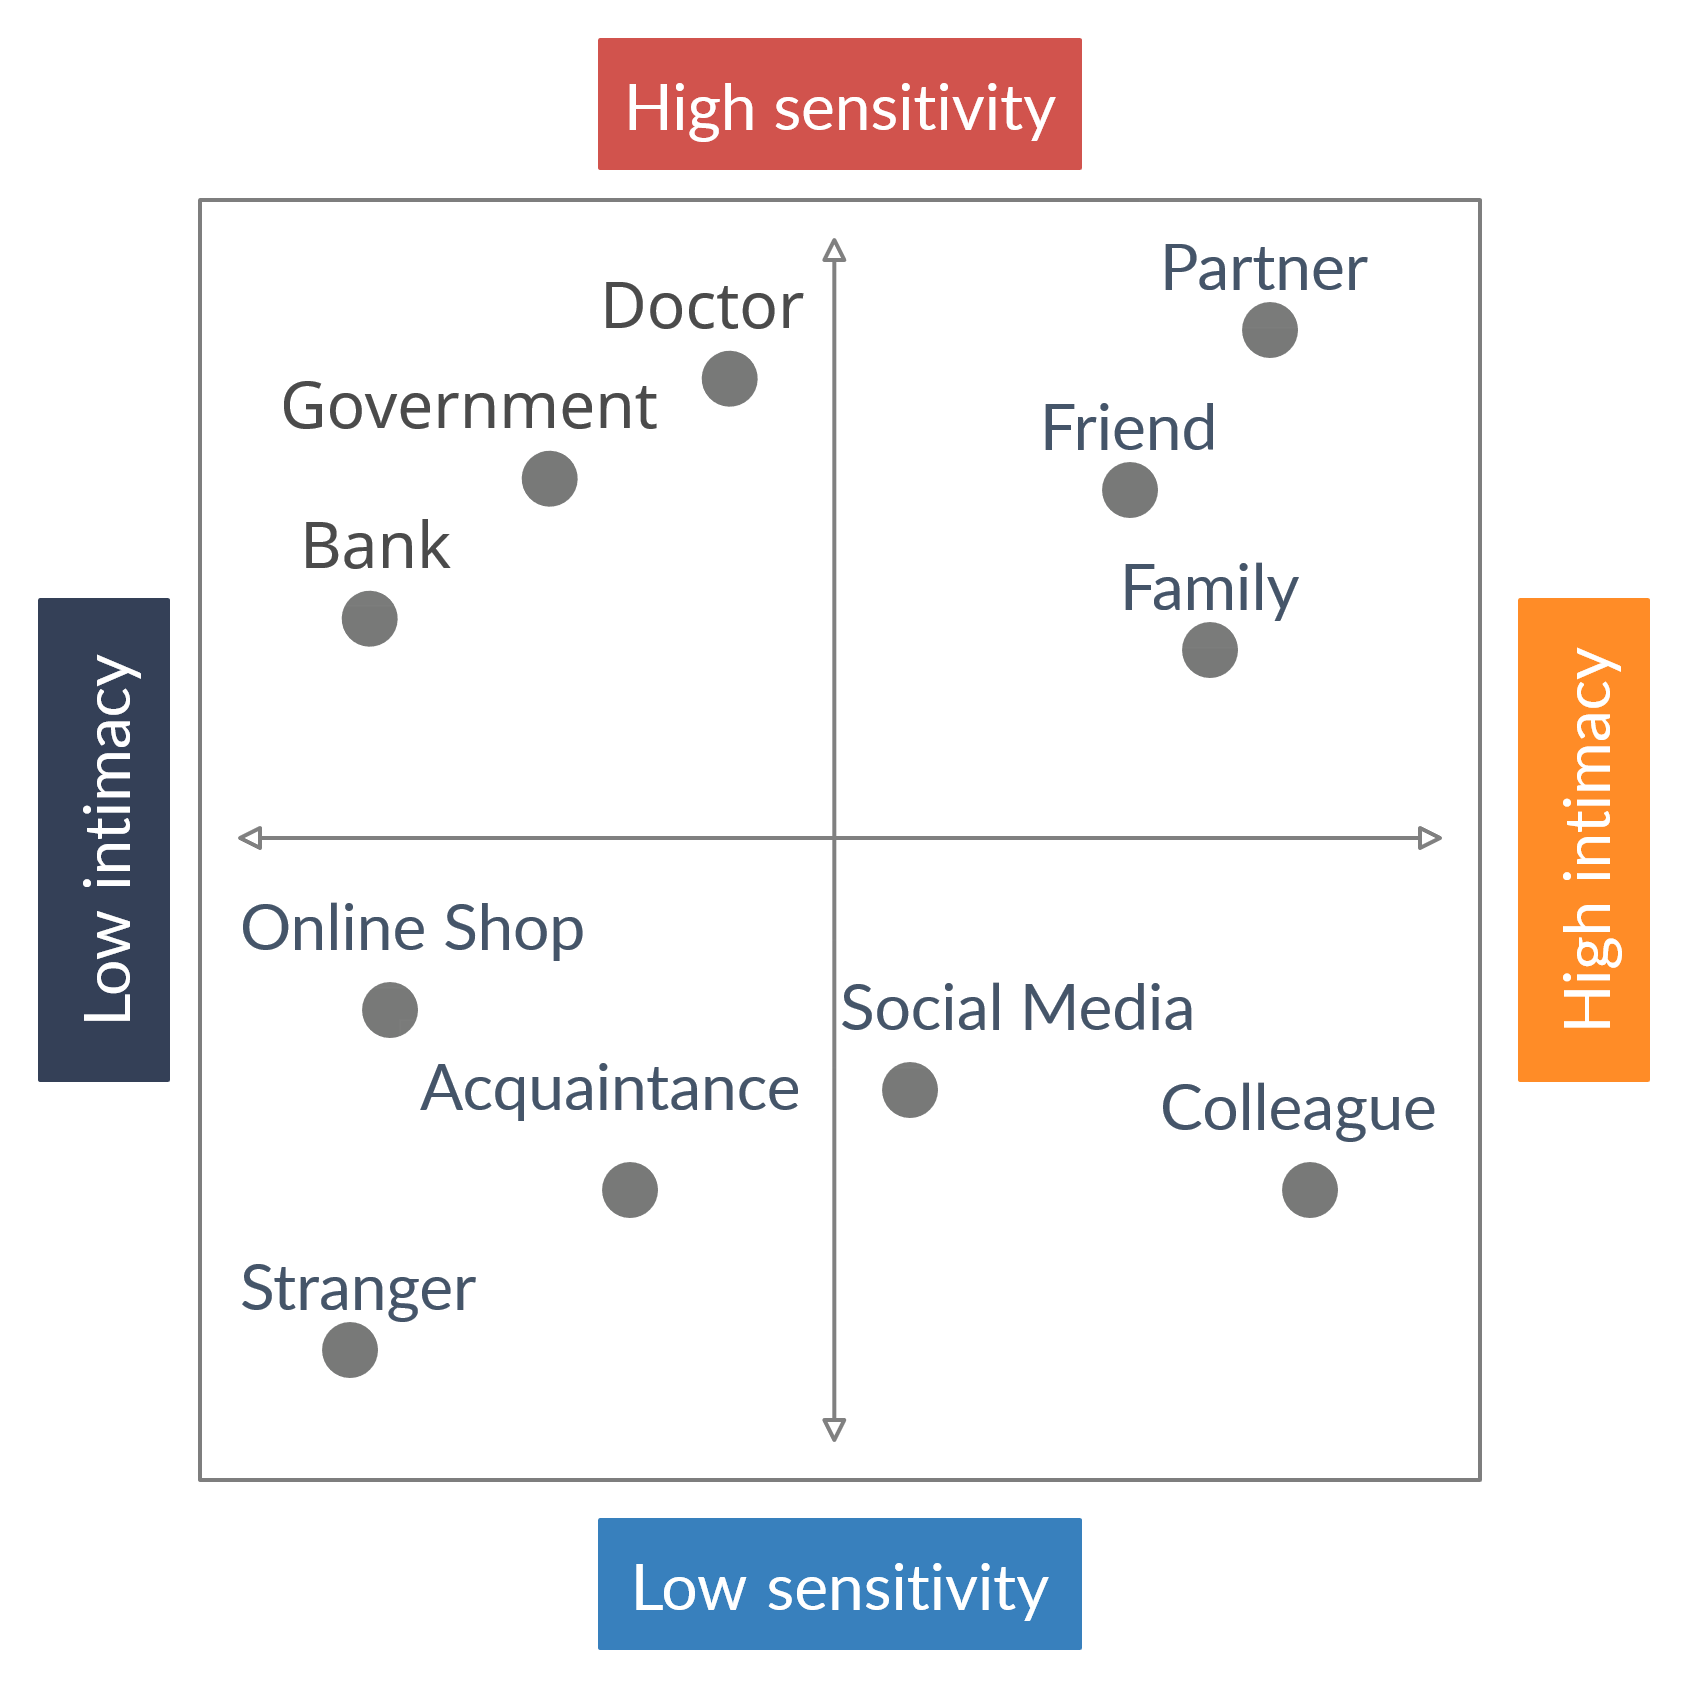
\includegraphics[width=\linewidth]{Personal Information intimacy vs sensitivity}
  \caption{Two possible dimensions of user control for personal identifiable information: sensitivity and intimacy, based on \cite{kim2018HowMultilevelPrivacy} and \cite{knijnenburg2013HelpingUsersInformation}.}
  \Description{Security risks of personal information}
  \label{fig:sensitivityvsintimacy}
\end{marginfigure}

The source of information to be used for personalization can be based on previous conversations or on user information and preferences that were explicitly encoded prior to the user-agent conversations. %In this paper we focus on one particular aspect of personalization, namely the creation of a user profile containing personal and possibly uniquely identifiable information of the user. 
Personalized conversational agents that allow for free language input are still rather uncommon. \citeauthor{Montenegro2019surveyagents} performed a systematic literature review (March 2019) and one of observations was that user consent for information collection needs more attention. \cite{Montenegro2019surveyagents}. %quote:\citeauthor{Montenegro2019surveyagents} "implicit methods used for gathering user information need to be clearly communicated to the users, since such methods often run automatically in the background, not being noticed by users. To this end, the model of informed consent for information systems may prove useful for considering various factors involved in collecting personal information"
%\citeauthor{kocaballi2019personalization}  personalized conversational agents in the health care domain that allow for free language input and were properly evaluated with users. They only found 13 studies matching these criteria. Personalization is aimed a individuals (and not at groups), expressed at content level 


%%%%%%%%%%%%%%%%%%
% Privacy
%%%%%%%%%%%%%%%%%%
\subsection{User Privacy Control}
In our project \emph{Behaviour-based Language-Interactive Speaking Systems} (BLISS), self-disclosure of personal information plays an important role \cite{vanwaterschoot2020BLISS}. Personal identifiable data (PII) should be handled with absolute scrutiny. Personal information such as names, emails and age are part of PII. Additionally information about where people go shopping or which sports association they are a member can be PII as well. Over time, our CA develops a relationship with a person to let them open up more and share more personal information. However, not every person is eager to share this information because some people are less trustworthy of technology \cite{rapp2016PersonalInformaticsEveryday}. Privacy aware users often appreciate a system's ability to be involved in setting privacy preferences. A CA can for example justify to a user why it wants the user to self-disclosure, though this not always results in a user self-disclosing more, sometimes even on the contrary (see Figure \ref{fig:appy}) \cite{knijnenburg2013HelpingUsersInformation}. Additionally, users are inclined to share more sensitive information in the beginning compared to later in a conversation. Setting the self-disclosure threshold at a sensitive level already does help in the user self-disclosing more sensitive information later on according to \cite{knijnenburg2013making}.

\begin{marginfigure}
    \centering
    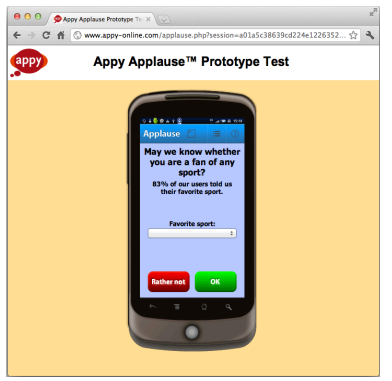
\includegraphics[width=\linewidth]{appy}
    \caption{An app that uses justification for asking PII from the user. \cite{knijnenburg2013HelpingUsersInformation}}
    \label{fig:appy}
\end{marginfigure}

Not all personal information is equally private.
% This is unclear: and is heavily dependent on context
\citeauthor{kim2018HowMultilevelPrivacy} defined multiple levels of private information, depending on the needs of the users \cite{kim2018HowMultilevelPrivacy}. People are willing to share their favorite color and name of first pet much more likely than a voice signal or email
% This is unclear: the sensitivity of the information.
\cite{marmion2019WillingnessCrowdsCohort}. Additionally, users prefer to share the most sensitive PII only with people they are intimate with (immediate family) or people who need it (doctors) \cite{rapp2016PersonalInformaticsEveryday}. In Figure \ref{fig:sensitivityvsintimacy}, we plot two dimensions of sensitivity and intimacy regarding PII. Interestingly, users can also delegate the control of their PII to third parties they trust, such as friends, experts or even AI \cite{nissen2019ShouldAgreeDelegating}. Depending on the context, different information is delegated to third-parties, for example health information to their general practitioner.

%We focus on personalized long-term engaging conversations with elderly people to collect and reflect on their overall health and well being \cite{vanwaterschoot2020BLISS}. We are not so much interested in clinical health but in a broader concept of well being and happiness that also comprises concepts such as quality of life, social participation and the overall capability to self-manage\cite{Huber2011}.
% The use of conversational agents in health care is growing \cite{Montenegro2019surveyagents}.
%Several studies have been conducted to check for the widespread acceptance of such technology in health care.
%\citeauthor{health-counseling2020} conducted such a study and concluded that mothers prefer counselling when done through conversational agents rather than other mediums \cite{health-counseling2020}.
%The study also showed that women prefer conversation agents as an effective, safe, and non-judgmental way of communication.
%\citeauthor{zahra2019} have designed a dialogue manager to conduct conversations with with older adults in order to receive feedback on their non-verbal communication such that to improve their communication skills \cite{zahra2019}.
%\citeauthor{Abdollahi2017} have showed the use of social robots in elderly homes to help patients in long-term engagements with robots and to improve the quality of their life specifically in patients having dementia and depression.
%They also incorporated humor and other features that make robots likable for longer interactions so that subjects interest is intact for longer period of time \cite{Abdollahi2017}.

%On the technological aspects of the CAs in the health care, there are also numerous studies.
%\citeauthor{oliveira2017speaking} conducted several studies and evaluated their results to check the technical aspects of speech technology namely speech recognition and speech synthesis \cite{oliveira2017speaking}. They found that although the speech technology performs well in many condition, but for elderly people several challenges arises.
%These include inadequate speech quality from the elderly people due to speech impairments related to age, speaking style and recognition problems that arises due to distance speech.
%\citeauthor{vanwaterschoot2020BLISS} also showed some issues that arises in the spoken dialogues.
%In order to have improved technology that performs well for a broader and variety of audience, the technology must be personalised to a particular person.
%Also the type and content of the conversations should be of interest to the users.
% Designing conversational agents To design more personalised conversational agents, more information and data needs to be acquired, and the person using the system needs to consent to give such information.
%For the speech recognition perspective this means the acoustic characteristics of the persons needs to be store in a system so that the voices are better recognized. 
%And for the speech synthesis point this means that preference of the synthetic voice (agent voice) needs to be adhered to the preferences of the user. 
%This could involve age, dialect and gender of the selected agent voice. %This could also include informing the agent about an important person in the subjects life.

%The personalization of the conversational agents no doubt provide an intimate and having a companion feeling to the user. 
%However, to have a personalized conversation agents, one needs to disclose personal information that some of us might hesitate to reveal.
%Specifically, for the design of the dialogues, if the conversation agents ask about previous life experience, accidents, any particular disease or some other events. 
%This type of personal information is required by the agent to give a close companionship feeling to the user.
%But most of us afraid to reveal such information and rightly so because revealing such information can have a negative social impact on the users life.
%In the section below, we briefly state what personalization is and give a brief overview of the work done in this direction. 

%The users of the system are very concern in the privacy and confidentiality of their medical and personal information.
%\emph{Privacy} can be defined as the right and desire of a person to control the disclosure of personal health information.
%To ensure the privacy of the user, proper policies and procedures needs to be maintained so that the information is accessible but only to the one whom the user of the system have given consent.


Existing technology, especially in recommendation systems, have researched different ways of providing informed consent and control of PII by users. However, in spontaneous conversations with CAs we have yet to go beyond the standard informed consent form. We argue that a single consent form signed prior to the user-agents conversations is insufficient for long-term interactions and recommend novel ways to provide transparency.


% Other possible options, solutions:
% ** Profile moet altijd beschikbaar zijn voor de gebruiker + 'kring' [familie, mantelzorgers, ...],
% de gegevens moeten op een duidellijke manier gepresenteerd worden,
% en de gebruiker moet kunnen 'editten' - alles kunnen verwijderen
% ** Or: sensible info. is stored locally, on the device of the user ?

\section{Transparency in Personal Identifiable Information} 
In work on spoken dialogue systems we observe a fundamental conflict between restrictions imposed by privacy regulations on the one hand, and personalization as a feature of the interaction on the other. Obviously this paradox is not limited to CAs and has been discussed for other applications as well \cite{awad2006personalization}. As we aim to develop agents that have previous knowledge about their interlocutors and are capable of adapting to their needs, we need to explicitly model personal profiles and store information from previous conversations. Personalization also contributes to long-term engagement and is crucial for establishing credibility and trust of the CA, which in turn are essential for actually having an effective CA that can provide insights in personal health and even stimulate behavioural change like in coaching and counseling agents. Trust appears to be an essential element of long term conversational engagement \cite{Bickmore2005} as is needed in health related CAs. A personalized CA that has knowledge about previous conversations helps building such trust.

All this might be difficult to reconcile with privacy regulations that were introduced to protect personal data such as GDPR, which require that information should not be traceable. So, for each piece of personal information that is incorporated in the CA, users need to give previous explicit consent, which is excellent, but also makes the procedure lengthy and tedious. 
As we create conversational agents for research projects, we follow the regulations of proper research ethics and give participants a clear explanation of the research they engage in followed by signing a consent form, a necessary step. After giving consent, the user no longer has any influence on what is stored from the conversations.
However, explicit consent given upfront may not be sufficient. Users should also remain in control of their own easily accessible data.
% This is unclear: especially when deployed in the field.

It is clear that storing all this sensitive information also poses enormous challenges in terms of safety and security. This might be less of problem when large health providers are involved, but for individual users this could just be a bridge too far. %JW: Depends, I don't want the health insurance provider to know everything, but I do like my GP to know stuff.
The security issue emerged clearly during the COVID19 crisis which caused a shift to online solutions that are much more vulnerable. In our BLISS project, the effects of the pandemic led to an unexpected struggle. We had developed a software architecture that works on device, but this could not be used because we were not allowed to conduct experiments on the premises. We switched to an online version, which was dependent on commercial video call services and is more prone to privacy breach in terms of security.


%%EXAMPLE OF CONFIGURABLE IN RECOMMENDER SYSTEMS
\section{Proposed solutions}
A possible way for users to take back control is the following: At the end of each (part of a) dialogue they can see the information collected, and decide what can (not) be stored in their profile.
The form of such mechanism is highly dependent of the CA architecture and its target users. For online text-based chatbots with a structured dialogue architecture, the template of stored personal information by the agent can be displayed as an online form that the user can then adapt to control which personal information is accessible by the agent. Natural language generation can be used to convert the structural data of such a form into a more natural language representation that is understandable by the user. However, giving consent after each exchange has a detrimental effect on long-term user engagement.

Another useful feature for control would be to establish layers of accessibility for personal data, such that the information contained in the CA is accessed to different degrees by different individuals like the users themselves, their family and/or care providers \cite{kim2018HowMultilevelPrivacy}. \citeauthor{marmion2019WillingnessCrowdsCohort, rapp2016PersonalInformaticsEveryday} found that depending on the context of an application, end-users are willing to disclose different types of personal information \cite{marmion2019WillingnessCrowdsCohort}.

A particular problem for end-users about their personal information is that current technology's feedback is often confusing with complex, excessive graphs \cite{rapp2016PersonalInformaticsEveryday}. A solution for spoken dialogues that we propose is to use summarized content reflection at the end of a conversation as a mechanism for user control and feedback \cite{razavi2019dialogue}. Automatic abstractive conversational summarization is a challenging new task \cite{zhao-2020-improving} that might provide an elegant solution to create such summarized content.

%iris:
% This table \ref{tab:freq} only if we have time and space to discuss some long-term engaging CAs in health and the possible mechanism solution for user consent at different stages. 
% \begin{margintable}
%   \caption{Architectures and Solutions}
%   \label{tab:freq}
%   \begin{tabular}{cc}
%     \toprule
%      example case & solution\\
%     \midrule
%     BLISS - Spoken information states & \\
%     Written template based & \\
%     rdf triplets &\\
%     RASA example & \\
%   \bottomrule
% \end{tabular}
% \end{margintable}

\section{Summary and conclusion} 
For CAs, the combination of personalization and privacy is problematic. The development of efficient and user-friendly CAs requires knowledge of the user, and as a consequence personal user profiles and information from previous conversations must be stored and re-used in a flexible way. Since this may include sensible (e.g. medical) data, privacy is a matter of utmost concern. 

All bits of personal information stored in the system needs a form of consent, preferably explicitly by the user instead of implicitly by e.g. agreeing on embarking on a conversation with a CA. In addition, controlling the data and accessibility of persona data is an aspect that needs careful consideration, both in the design and architecture of the system but also (and, even more importantly) in the information flow along the entire data path during interaction, especially in the case where external web services are employed for the online functioning of the CA.

We argued that static and dynamic management by the user of stored personal information within agents can provide an adequate and powerful solution for resolving the privacy versus personalization conflict.

%%
%% The acknowledgments section is defined using the "acks" environment
\begin{acks}
This work is part of the research programme Data2Person with project number 628.011.029, which is (partly) financed by the Dutch Research Council (NWO). 
\begin{marginfigure}
%\begin{flushright}
    
\includegraphics[width=20mm]{NWO-logo.png}
%\end{flushright}
\end{marginfigure}
%todo
\end{acks}
%\vspace{-7mm} % louis here some more tex

%\vspace{-10mm}
%%
%% The next two lines define the bibliography style to be used, and
%% the bibliography file.
\bibliographystyle{ACM-Reference-Format}
\bibliography{BLISS}

\end{document}
\endinput
%%
%% End of file
